% !TEX root = ../main.tex

\chapter{主要研究内容及研究方案}

\section{研究内容}

\subsection{存储编码的基本原理}

纠删码是一类通过冗余编码提升数据可靠性的算法，可作为存储编码应用到存储系统中，相比于创建多个数据副本以防数据丢失，它通过数学算法将原始数据转换为带冗余信息的编码数据，在可靠性与存储效率间取得平衡，非常适用于大规模分布式存储场景。以最经典的Reed-Solomon（RS）码\cite{reedPolynomialCodesCertain1960}为例，假设将原始数据均分成$k$个数据块，再同生成矩阵进行有限域上的矩阵乘法运算，编码出$m$个校验块，总计得到$n=k+m$个块，并将这$n$个块分别存储到$n$台分布式的存储设备中，这样最多能容忍$m$块数据丢失，即$m$台设备故障。RS码的编码过程可由\equref{equ:RSEncode}表示。

\begin{equation}
    \mathbf{C} = \mathbf{G} \times_{GF[2^w]} \mathbf{D}
    \label{equ:RSEncode}
\end{equation}

其中，$\mathbf{D}$为原始数据块向量，$\mathbf{G}$为生成矩阵（通常为Vandermonde或Cauchy矩阵\cite{lubyXORBasedErasureResilientCoding1995}），$\mathbf{C}$为编码后的校验块向量。\figref{fig:RSEncodeExample}以$k=4, m=3$为例，展示了RS码的编码过程。

\begin{figure}[htbp]
    \centering
    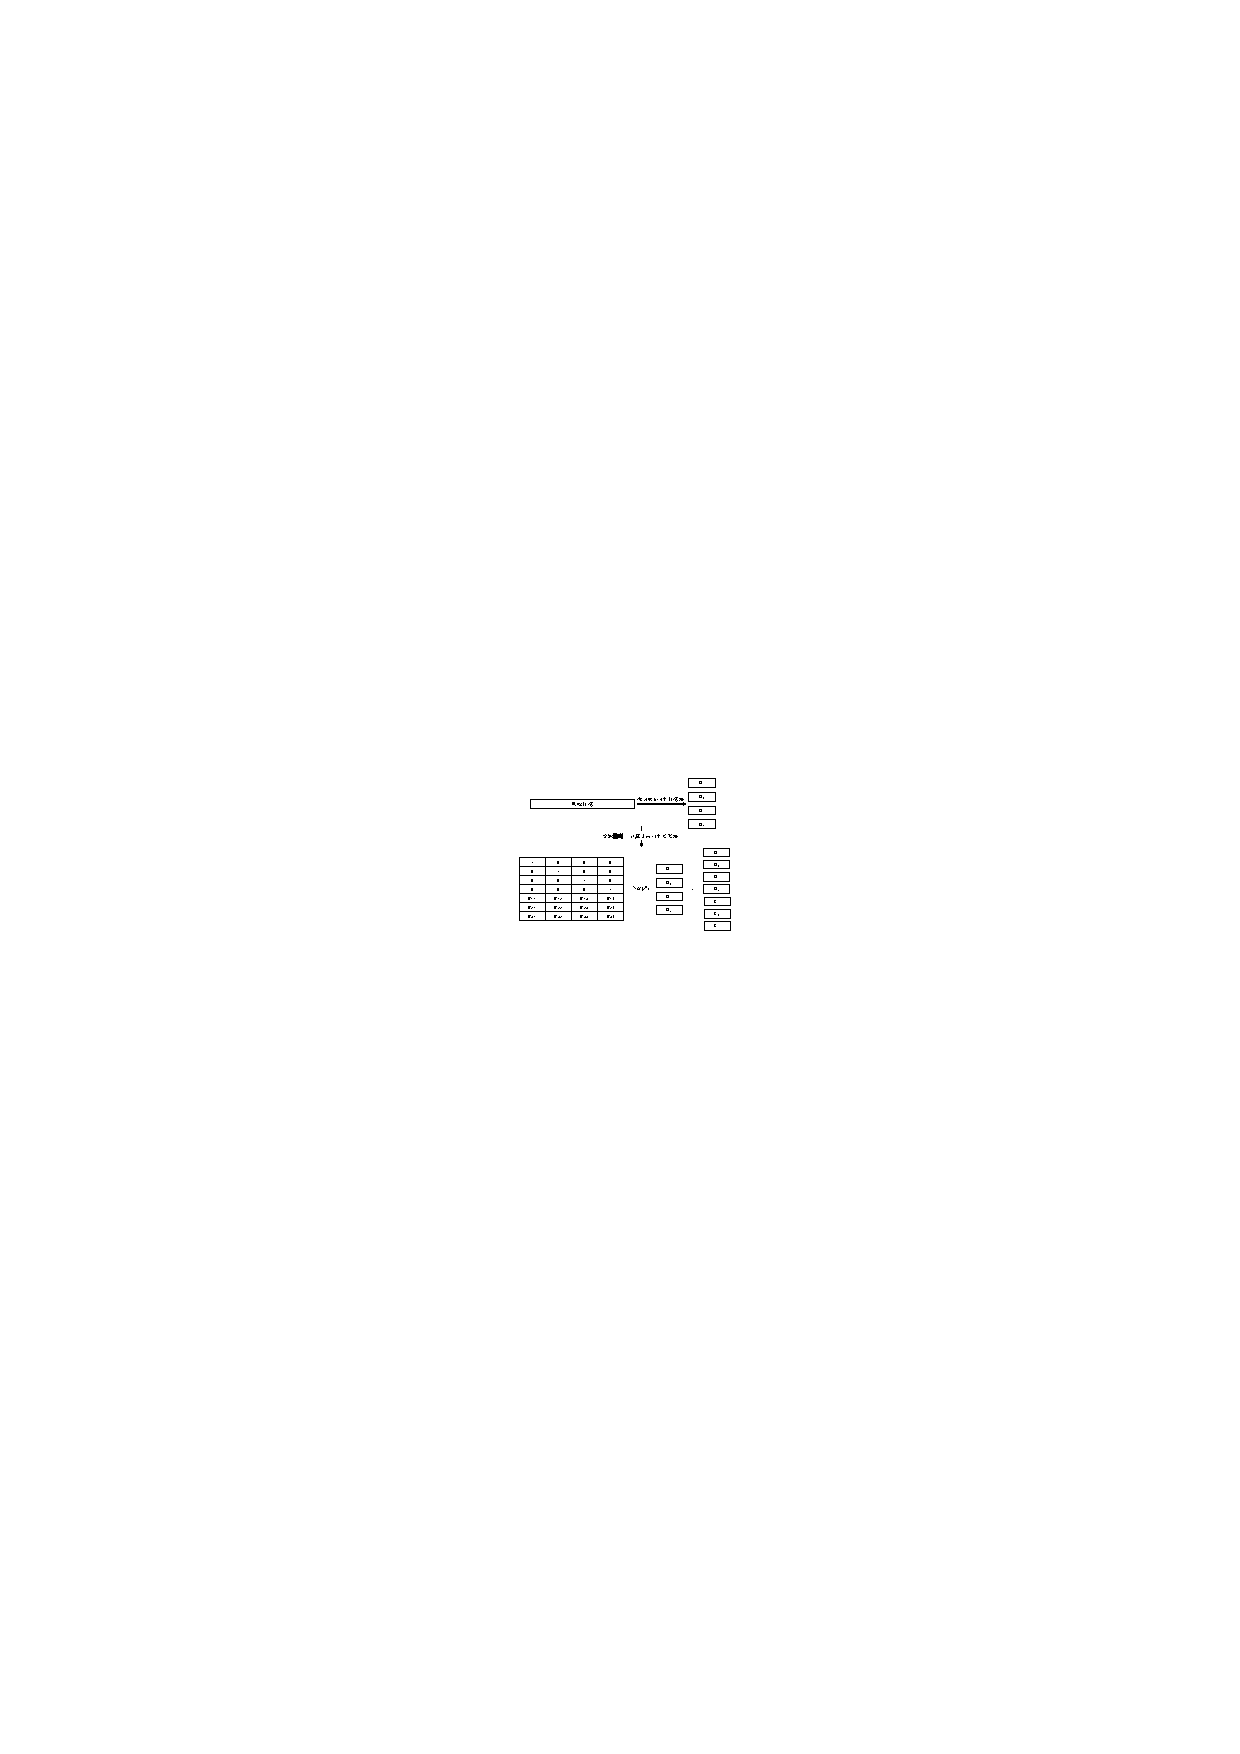
\includegraphics[width=0.7\textwidth]{figures/RS码编码举例.pdf}
    \caption{RS码编码举例}
    \label{fig:RSEncodeExample}
\end{figure}

解码时，根据丢失数据块的情况，基于编码公式构造逆矩阵，得出新的解码公式，从而恢复丢失的数据块，再重新编码以恢复丢失的校验块，可由\equref{equ:RSDecode}表示。

\begin{equation}
    \mathbf{D} = \mathbf{G'}^{-1} \times_{GF[2^w]} \mathbf{D'}
    \label{equ:RSDecode}
\end{equation}

其中，$\mathbf{D'}$为所有未丢失的数据块和校验块构成的向量，$\mathbf{G'}^{-1}$为根据丢失情况构造的逆生成矩阵，$\mathbf{D}$为原始数据块向量。\figref{fig:RSDecodeExample}以$k=4, m=3$为例，展示了RS码的解码和重编码过程。

\begin{figure}[htbp]
    \centering
    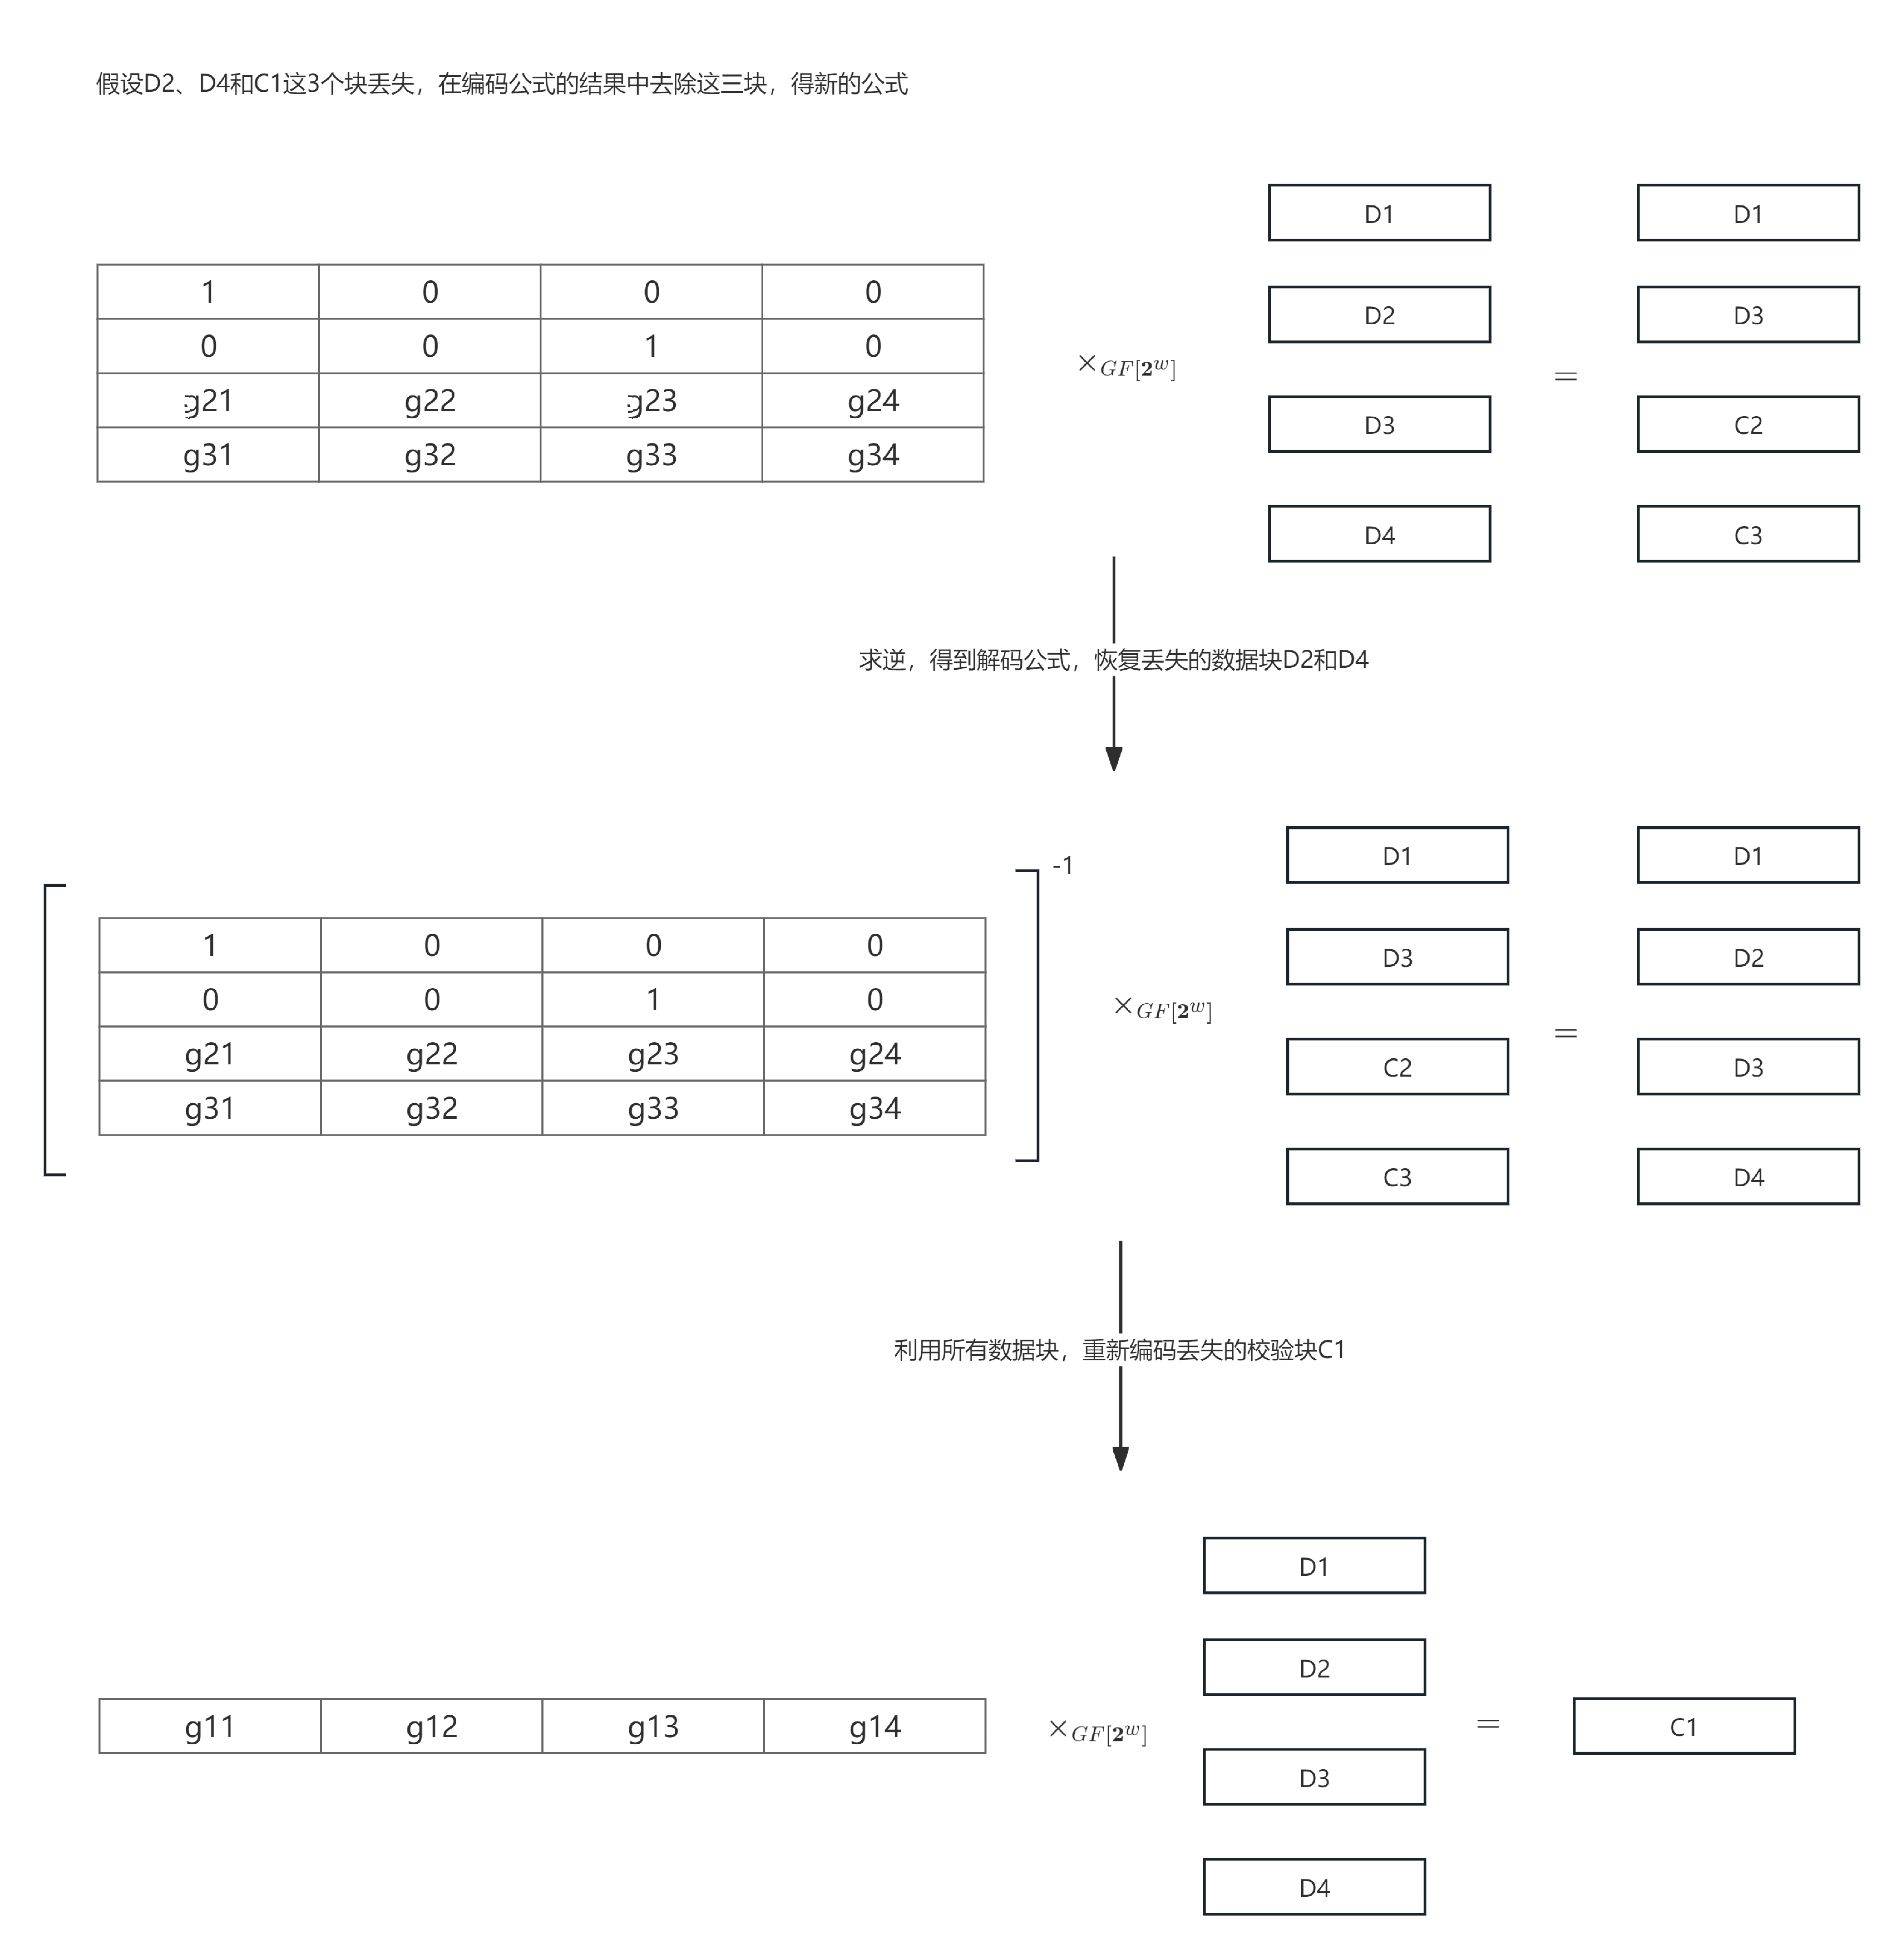
\includegraphics[width=0.7\textwidth]{figures/RS码解码举例.pdf}
    \caption{RS码解码举例}
    \label{fig:RSDecodeExample}
\end{figure}

\subsection{Two-tone Shift-XOR的编码原理}

Two-tone Shift-XOR码是一种基于移位和异或操作的高效纠删码。其核心思想是利用规则的移位矩阵和异或运算实现编码与解码，避免有限域上的乘法运算，提升运算效率。Two-tone码的编码过程可由\equref{equ:TwoToneEncode}表示。 

\begin{equation}
    \mathbf{C} = \mathbf{Z} \times \mathbf{D}
    \label{equ:TwoToneEncode}
\end{equation}

其中，$\mathbf{Z}$为移位生成矩阵，采用最简单且规则的Two-tone矩阵\cite{fuTwotoneShiftXORStorage2021}，其中每个元素$z^{s_{ij}}$代表偏移量。
假设原始数据块分别为$\{D_1, D_2, \dots, D_k\}$，编码后得到的校验块分别为$\{C_1, C_2, \dots, C_m\}$，则Two-tone的编码公式还可以表示为\equref{equ:TwoToneEncodeSingle}。

\begin{equation}
    C_i = \bigoplus_{j=1}^{k} z^{s_{ij}}D_j
    \label{equ:TwoToneEncodeSingle}
\end{equation}

其中$z^{s_{ij}}D_j$表示对数据块$D_i$进行$s_{i,j}$个单位的非循环移位，$\oplus$为异或操作。\figref{fig:RSEncodeExample}以$k=4, m=3$为例，展示了RS码的编码过程。



Two-tone算法的生成矩阵具有特殊结构，使得解码时可按序消除丢失块，提升解码效率。

% \begin{figure}[htbp]
%     \centering
%     \includegraphics[width=0.7\textwidth]{figs/twotone_matrix_example.pdf}
%     \caption{Two-tone Shift-XOR编码矩阵示意图}
%     \label{fig:twotone_matrix}
% \end{figure}

\subsection{优化问题描述}

尽管Two-tone Shift-XOR码在理论上具备高效性，但实际工程实现仍面临如下优化问题：
\begin{itemize}
    \item 如何统一处理所有丢失情况，实现解码泛化与高效性兼顾；
    \item 如何提升缓存局部性，减少内存访问压力；
    \item 如何在寄存器层面合并数据块，降低内存读写次数；
    \item 如何针对特殊丢失场景进一步特化优化，发挥硬件指令优势。
\end{itemize}

\section{研究方案}

\subsection{统一解码抽象：Erasure-Parity Mapping}

针对多样化丢失情况，提出erasure-parity mapping结构，将所有丢失块（数据块或校验块）统一抽象为erasure结构。每个erasure结构按编号匹配丢失块，数据块优先，校验块后置。对于数据块丢失，寻找对应校验块进行解码；对于校验块丢失，则重新编码。若丢失块数小于阈值，则无需处理。该结构实现了解码流程的统一抽象，简化了条件分支。

% \begin{figure}[htbp]
%     \centering
%     \includegraphics[width=0.7\textwidth]{figs/erasure_parity_map.pdf}
%     \caption{Erasure-Parity Mapping结构示意图}
%     \label{fig:erasure_parity_map}
% \end{figure}

\subsection{缓存友好窗口划分：Cache-Friendly Window}

为提升缓存局部性，将较长的数据块（chunk）划分为较小的窗口（window）进行处理。每个window独立初始化，仅在首次访问时进行计算（init on first access），并采用局部异或写入校验块。该方法有效减少缓存失效和初始化开销。

% \begin{figure}[htbp]
%     \centering
%     \includegraphics[width=0.7\textwidth]{figs/cache_window.pdf}
%     \caption{Cache-Friendly Window处理流程}
%     \label{fig:cache_window}
% \end{figure}

\subsection{内存友好邻域合并访问：Neighbor Merging Access}

编码时，数据块访问有横向（逐块）和纵向（逐slice）两种模式。横向访问集中处理数据块，纵向访问则针对校验块slice。提出邻域合并策略，将相邻两个数据块chunk在寄存器中合并处理，纵向运算后再写入校验块内存，理论上减少约50\%的内存访问。

% \begin{figure}[htbp]
%     \centering
%     \includegraphics[width=0.7\textwidth]{figs/neighbor_merging.pdf}
%     \caption{Neighbor Merging Access编码模式示意}
%     \label{fig:neighbor_merging}
% \end{figure}

\subsection{特化与泛化结合：Special Case Expansibility}

虽然解码流程已实现泛化，但针对特殊丢失场景（如仅丢失一个块），可进一步特化优化。例如，移位异或特性允许直接异或全部chunk恢复丢失块，无需zigzag逐步解码。此时可利用AVX2流指令，提升解码效率。特化与泛化结合，使解码在全场景下均具备高效方案。

% \begin{figure}[htbp]
%     \centering
%     \includegraphics[width=0.7\textwidth]{figs/special_case.pdf}
%     \caption{特化场景下的高效解码流程}
%     \label{fig:special_case}
% \end{figure}